% Logarithmic spiral
% Author: Andrew Mertz
\documentclass{minimal}
\usepackage{tikz}
\usetikzlibrary{backgrounds,calc}
\begin{document}
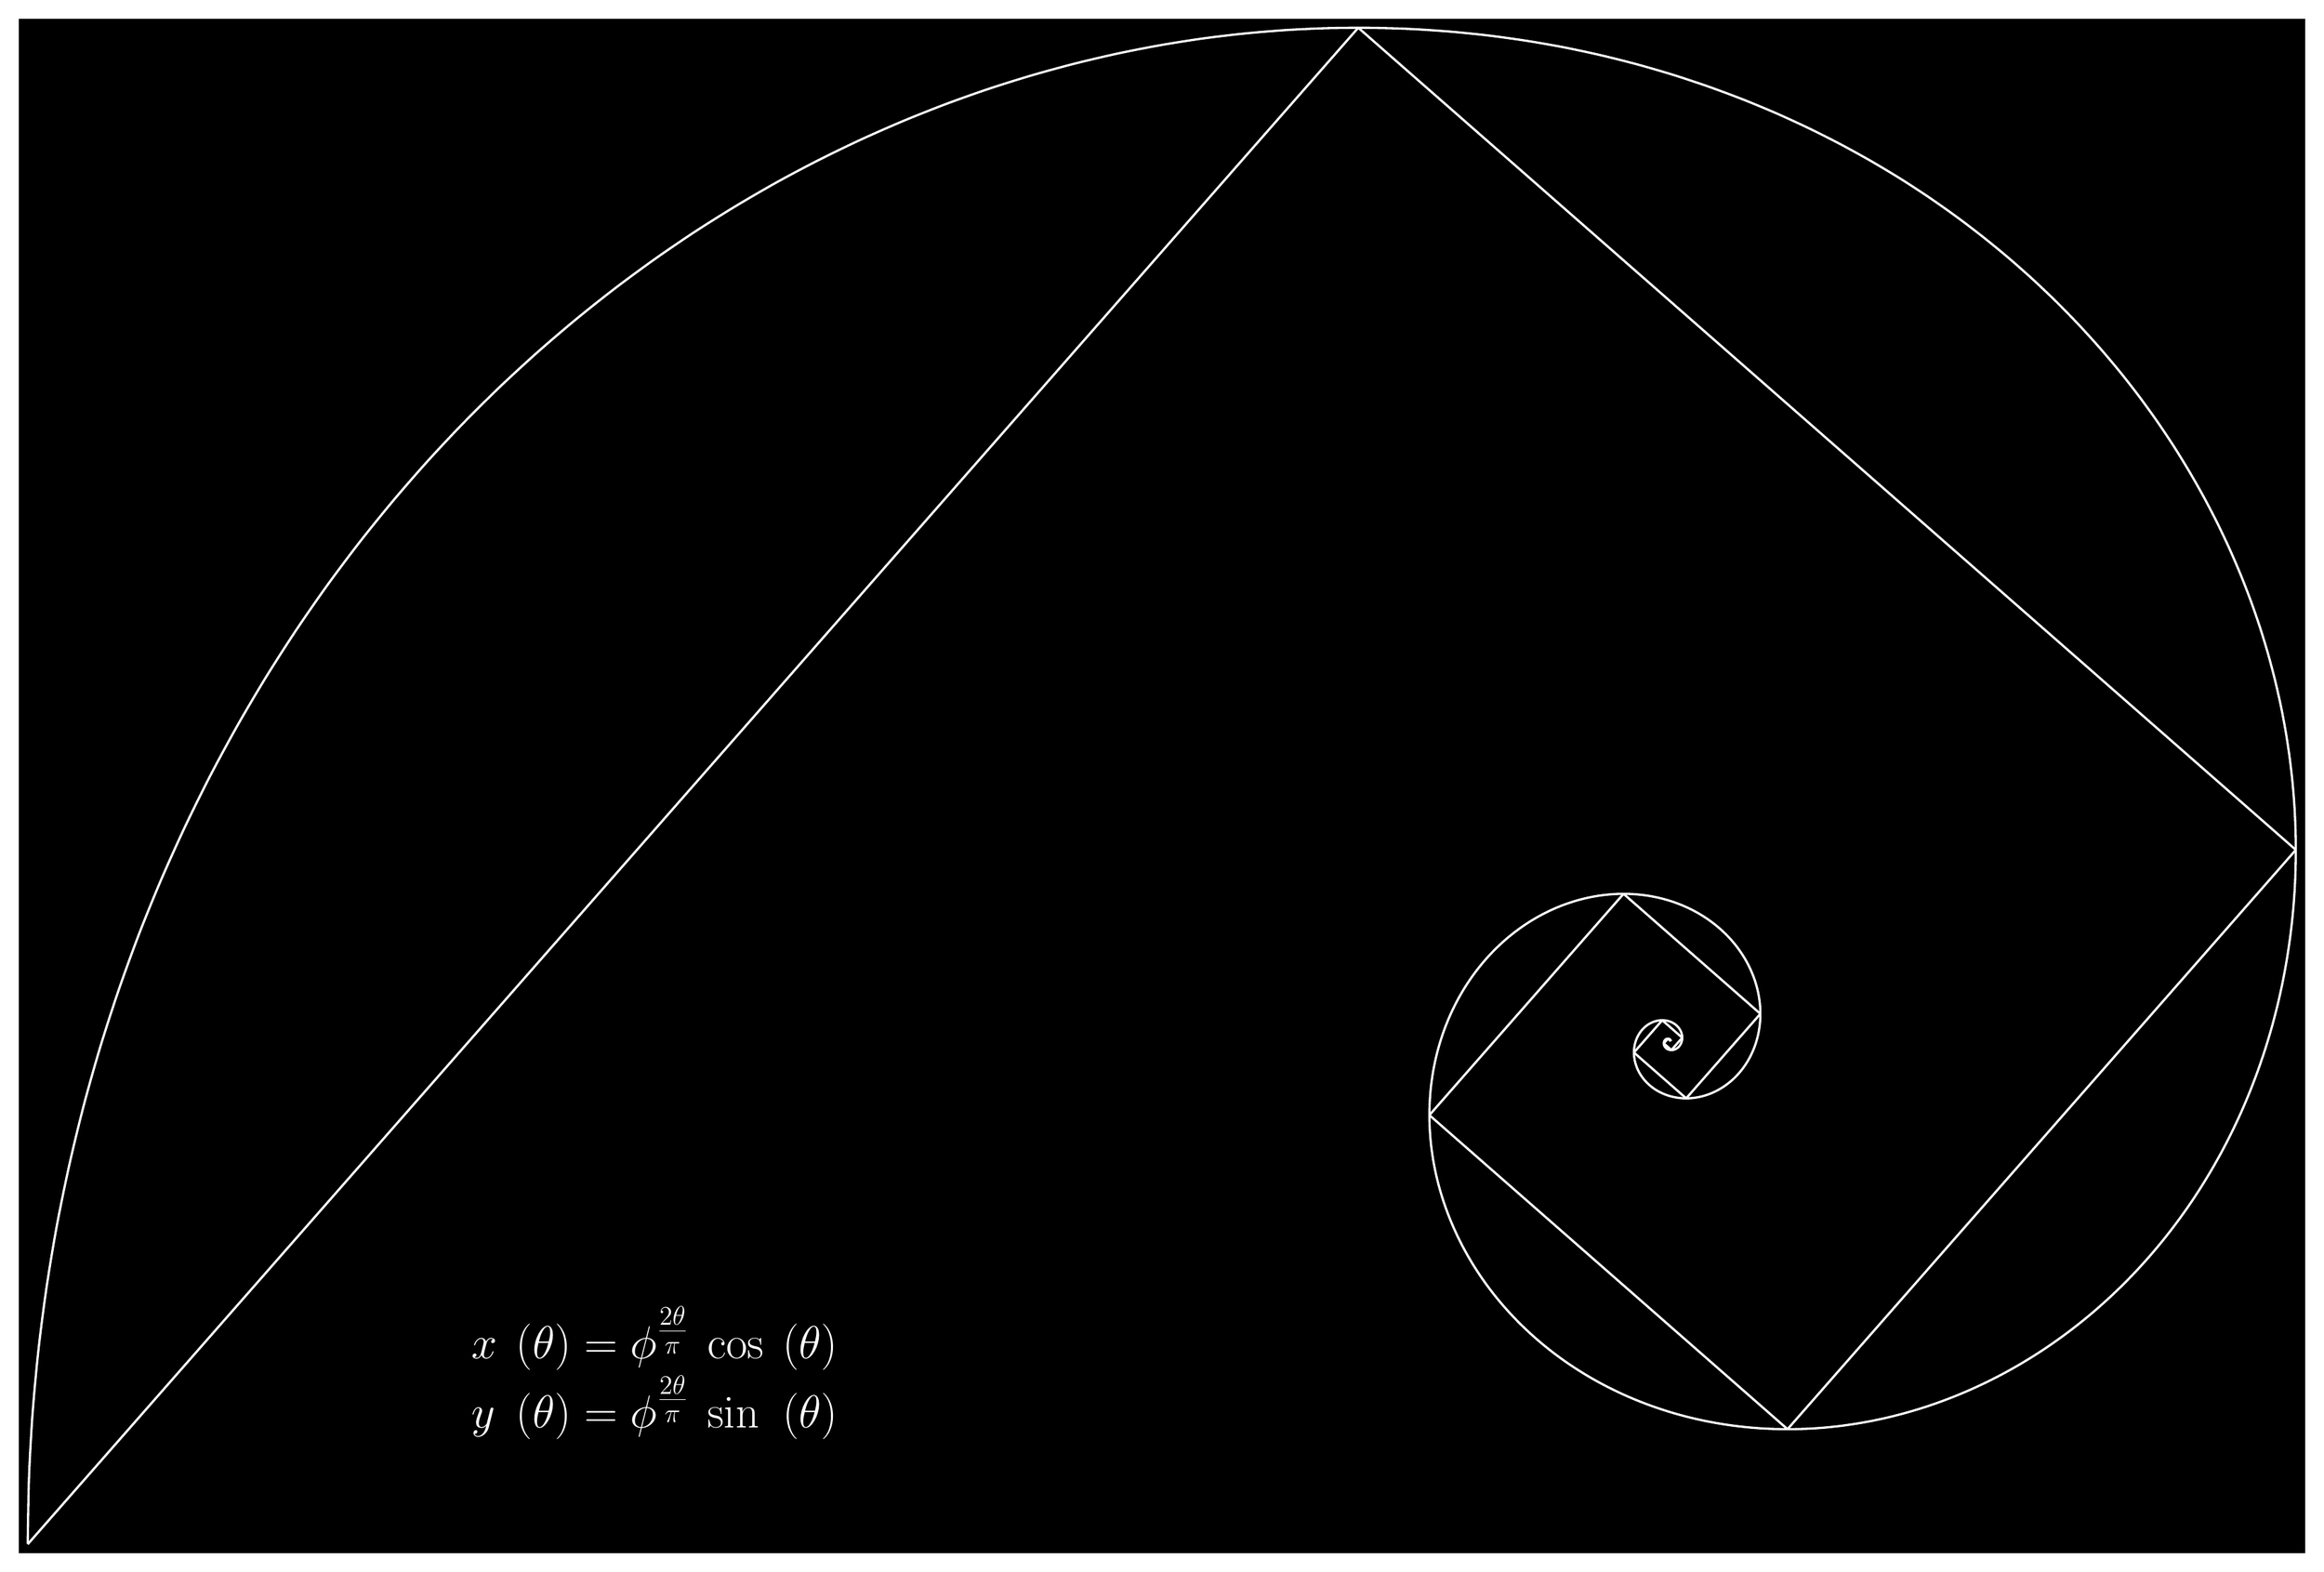
\begin{tikzpicture}[background rectangle/.style={fill=black},
                    show background rectangle, x=1pt, y=1pt]
 % Compute the golden ratio
  \pgfmathsetmacro{\goldenRatio}{(1+sqrt(5)) / 2}

  % Compute the angle between the tangent and radial line 
  \pgfmathsetmacro{\offset}{rad(atan(2*ln(\goldenRatio)/pi))};

  % Plot the spiral using the parametric form of a logarithmic spiral
  % (a e^{b t} cos(t), a e^{b t} sin(t)). In this case a = 1 and b = 2
  % ln((1+sqrt(5)) / 2) / pi. There can be a slight gap between the
  % last line segment and the end of the plot. Having a large sample
  % size reduces the gap.
  \draw[very thick,white,domain=\offset:\offset+14*pi/2,
       smooth,samples=600,variable=\t] plot
   ({pow(\goldenRatio, 2 * \t / pi) * cos(\t r)},
    {pow(\goldenRatio, 2 * \t / pi) * sin(\t r)}) 
   coordinate(end);

  % Remember the start of the spiral
  \coordinate (0) at 
    ({pow(\goldenRatio, 2 * \offset / pi) * cos(\offset r)},
     {pow(\goldenRatio, 2 * \offset / pi) * sin(\offset r)});

 % This loop draws the line segments
  \foreach \i in {1,...,14}
  {
    % Get the "name" of the last point on the spiral
    \pgfmathsetmacro{\lastpoint}{\i-1}

    % Compute the start angle for this turn of the spiral
    \pgfmathsetmacro{\angle}{\i * pi / 2  + \offset}

   \draw[very thick,white] (\lastpoint) --
     ({pow(\goldenRatio, 2 * \angle / pi) * cos(\angle r)},
      {pow(\goldenRatio, 2 * \angle / pi) * sin(\angle r)})
     coordinate (\i);
  }

  % Add some text displaying the formula for the parametric form of the
  % spiral
   \node(eq) at ($(14) + 5*(\goldenRatio cm,1cm)$) 
     [white,text width=2cm,font=\fontsize{30}{30}\selectfont,
      anchor=north west] {
     \begin{displaymath}
       \begin{array}{llll}
         x&(\theta) = \phi^{\frac{2\theta}{\pi}}&\cos&(\theta)\\
         y&(\theta) = \phi^{\frac{2\theta}{\pi}}&\sin&(\theta)\\
       \end{array}
     \end{displaymath}
  };
\end{tikzpicture}
\end{document}
% LocalWords:  tikzpicture TikZ sqrt ln atan eq llll
